

In this section we answer the two questions raised in Section~\ref{sec.motive} to conceptualize \textsc{Dms}.

\subsection{Identify High Change-potential Elements}

In order to evaluate the change-potential of program elements, we first represent program element's rank changes as time series data points. We then fit the points to a linear model using regression analysis. The regression coefficient of the model and the error (i.e., discrepancy between the model and the real points) are used as proxy to identify program elements with high change-potentials. More details are described as follows.

\vspace{0.2cm}
\noindent{\em Representative Time Series Construction.} We capture changes in the ranks of a program element as a series of {\em trend units}:

\begin{enumerate}
%	\setlength{\parskip}{0pt}%
    \setlength{\itemsep}{3pt}%
	\item When the rank of the program element decreases, its current trend unit is \texttt{[+]}.
	\item When the rank of the program element increases, its current trend unit is \texttt{[-]}.
	\item If the element's rank stays the same, its current trend unit is \texttt{[0]}.
\end{enumerate}

For example, the ranks of statement $s_{8}$ in different iterations and its corresponding trend units are listed in Table \ref{tab:trend_example}. This series of trend units is further converted to a series of points $<x_{i},y_{i}>$, where $x_{i}$ represents the iteration number, and $y_{i}$ represents cumulated changes in program ranks at iteration $i$. We set $y_{0}$ as 0. When the trend in iteration $i$ is {\bf \texttt{[+]}}, $y_{i} = y_{i-1} + 1$.
If the $i$-th trend is {\bf \texttt{[-]}}, $y_{i} = y_{i-1} - 1$, otherwise, if the trend does not change({\bf \texttt{[0]}}) then $y_{i} = y_{i-1}$. We refer to this series of points as the {\em evolution trend} of the corresponding program element.

\begin{table}[!h]
%	\small
	\centering
	\caption{Evolution Trend of $s_8$.}
	\renewcommand{\arraystretch}{1.5}
	\newcolumntype{C}{>{\centering\arraybackslash}m{0.45cm}<{}}
	\begin{tabular}{cCCCCCCCC}
		\hline
		Iteration ($x_{i}$) &1 &2 &3 &4 &5 &6 &7 &... \\
		\hline\hline
		Rank &11 & 6 & 4 &2 &3 &11 & 5 & ... \\
		Trend ($\mathcal{T}$) & {\bf}&{\bf\texttt{[+]}}&{\bf\texttt{[+]}}&{\bf\texttt{[+]}}&{\bf\texttt{[-]}}&{\bf\texttt{[-]}}&{\bf\texttt{[+]}}&... \\
		$y_{i}$ & 0 & 1 & 2 & 3 & 2 & 1 & 2 & ... \\
		\hline
	\end{tabular}
%	\vspace*{-8pt}
    \label{tab:trend_example}
\end{table}


\vspace{0.2cm}
\noindent{\em Linear Model Construction.} Then we use {\em linear regression analysis}~\citep{GrIy94} to model the trend of each program element. Each trend is modeled as a linear equation:

\begin{equation}
	y_{i}=\beta_{1}\cdot x_{i} + \beta_{0} + \epsilon_{i}
\end{equation}

\begin{comment}
\hide{
where the parameter $\beta_1$ is estimated by:
\begin{equation}
	\hat{\beta}_{1} = \frac{\sum\limits_{i}{(x_{i}-\bar{x})\cdot(x_{i}-\bar{x})}}{\sum\limits_{i}{(x_{i}-\bar{x})^2}}
\end{equation}
the error of estimation $\hat{\beta}_{1}$ is given by:
\begin{equation}
	\hat{\sigma}_{\beta_{1}} = \hat{\sigma}_{\epsilon}\sqrt{\frac{1}{\sum\limits_{i}{(x_i-\bar{x}^2)}}}
\end{equation}
in the equation, $\hat{\sigma}_{\epsilon}$ is the estimate of constant variance of error term, which is
defined by:
\begin{equation}
	\hat{\sigma}_{\epsilon} = \frac{1}{N-2} \cdot \sum\limits_{i}{e_{i}^{2}}
\end{equation}
where $e_{i} = y_{i} - \hat{y}_{i} $ which is the error between the actual value and predicted value.
}
\end{comment}

\vspace{0.2cm}
\noindent{\em Change Potential Computation.} In order to speed up the overall evolution process, our approach needs to select next test case that keeps elements with monotonic trends (high change-potential trends) evolving their rankings. In other words, we do not care about changing elements' ranking with unstable trends. In order to identify those high change-potential elements, we need a metric to evaluate and compare trends of different elements. Here we define the change-potential of a program element with trend $\mathcal{T}$ as:

\begin{equation}
	\mathcal{W}_\mathcal{T} =  \left| \hat{\beta}_{1} \right| \cdot \frac{1}{\hat{\sigma}_{\beta_{1}}+1}\label{eq:trend_metric}
\end{equation}


$\hat{\beta}_{1}$ is estimated by {\em least squares} and $\hat{\sigma}_{\beta_{1}}$ is the error of estimating $\beta_{1}$~\citep{GrIy94}. In this metric, the numerator is the absolute value of the trend slope and the denominator considers the fitness of the regression model which represents the deviation of the actual value from the regression model.

\noindent\textbf{Rational of Equation \ref{eq:trend_metric}:} \textit{A good trend should have a larger slope as well as a smaller deviation from the linear model.}

In our empirical model, fast changing monotonic model has a bigger slope and thus gets a bigger numerator. Meanwhile a stable and monotonic trend has a smaller deviation from the linear model and thus gets a smaller denominator. Using this metric, our method isolates trends that evolve in a monotonous and stable way. Table \ref{tab:trend_exp} shows a few example trends and their change-potentials according to Equation \ref{eq:trend_metric}.

\begin{table}[!htbp]
	\centering
%	\vspace*{-8pt}
	\caption{Trend examples and their potentials}
		\renewcommand{\arraystretch}{1.5}
%		\small
        \begin{tabular}{|cc|ccc|}
			\hline
			 \multicolumn{ 2}{|c|}{$\mathcal{T}$} &     $\hat{\beta}_{1}$ &      $\hat{\sigma}_{\beta_{1}}$ &  $\mathcal{W}_\mathcal{T}$ \\
			\hline\hline
			 {\bf \texttt{[+]}} &  {\bf \texttt{[+]}} &          1 &          0 &          1 \\
			\hline
			 {\bf \texttt{[+]}} &  {\bf \texttt{[-]}} &          0 &      0.577 &          0 \\
			\hline
			 {\bf \texttt{[+]}} &  {\bf \texttt{[0]}} &        0.5 &      0.289 &      0.388 \\
			\hline
			 {\bf \texttt{[0]}} &  {\bf \texttt{[0]}} &          0 &          0 &          0 \\
			\hline
		\end{tabular}
	\label{tab:trend_exp}
\end{table}

\subsection{Speed up the Rank Change Process}

After evaluating the program elements according to their change-potentials, \textsc{Dms} will try to speed up the evolution trend of the program elements based on the change-potential($\mathcal{W}_{\mathcal{T}}$). First, program elements with the same suspiciousness scores are grouped together, they are termed as {\em suspicious group} in this paper. These suspicious groups are then assigned change-potential scores based on the change-potentials of their constituent program elements. When new test cases are added, based on the actual program elements that get executed, some groups can be broken into two. When this happens, the diversity of the suspiciousness scores increases in most cases. The goal of \textsc{Dms} is to select a new test case that breaks a group into two sub-groups where the overall change-potentials are maximized.

We calculate the potential of a group $g$ by summing up the potential of all program elements $d$ that
belongs to $g$.
\begin{equation}
	\mathcal{W}_{g} = \sum\limits_{d \in g}\mathcal{W}_{\mathcal{T}_{d}}\label{eq:elem_potential}
\end{equation}

where $\mathcal{T}_{d}$ is the change-potential of the program element $d$ based on the labelled execution trace profiles.

\noindent\textbf{Rational of Equation \ref{eq:elem_potential}:} \textit{Group with high change-potential elements should be given higher priority to break.}

We want to diversify the rankings of elements in the suspicious group that has a high change-potential score. To identify those high change-potential groups, we measure the sum of change-potential scores of its member elements.

The overall change-potential score of all suspicious groups($G$) are calculated as follows:
\begin{equation}
	\mathcal{H}_G = \sum\limits_{g_{i} \in G}{ \mathcal{W}_{g_i}^{2} }\label{eq:groupset_potential}
\end{equation}

To evaluate an unlabeled trace $t$, {\sc Dms} calculates the difference between the overall change-potential score of the current groups $G$ ($\mathcal{H}_G$) and the overall change-potential score of all groups when $t$ is added to the pool of labeled test cases ($G \Leftarrow t$), and chooses the test case that can maximize the difference as the next one for labeling.
\begin{equation}
	\operatorname*{arg\,max}_{t \in T_\mathcal{U}} \left\{ \mathcal{H}_G - \mathcal{H}_{(G \Leftarrow t)} \right\}\label{eq:select_metric}
\end{equation}

The new groups ($G \Leftarrow t$) and their change-potential $\mathcal{H}_{(G \Leftarrow t)}$ can be estimated based on $t$'s spectrum (i.e., the set of program elements hit by $t$) even when the pass/fail label for $t$ is unknown. Given an existing suspicious group, if a newly added test case $t$ only covers a subset of the group elements, this group may be broken into two: one contains the elements hit by $t$, and the other contains the elements uncovered by $t$. Then, each subgroup inherits a portion of the original group's change-potential proportional to its size. For example, suppose a group $g$ in $\mathcal{H}_{G}$ contains 2 elements, whose potentials are 0.4 and 0.6 respectively, and a new test case $t$ breaks $g$ into $g_{1}$ and $g_{2}$, each of which contains 1 element; then, the change-potentials $\mathcal{W}_{g_1}$ and $\mathcal{W}_{g_2}$ are both $\frac{1}{2}\times(0.4+0.6) = 0.5$.

\noindent\textbf{Rational of Equation \ref{eq:groupset_potential} and \ref{eq:select_metric}:} \textit{Test cases that breaks more groups with higher change-potential should be given higher priority.}

Equation \ref{eq:groupset_potential} measures the overall change potential score of all suspicious groups and its square form manifests the diversity of elements ranking. 
As an example, suppose there are two groups $g_{1}$ and $g_{2}$. Group $g_1$ has two high change-potential elements with change-potential score 0.3 and 0.4. 
Group $g_{2}$ has two low change-potential elements with change-potential score 0.1 and 0.2.
According to equation \ref{eq:groupset_potential}, $\mathcal{H}_G = (0.3+0.4)^{2} + (0.1 + 0.2)^2 = 0.58$. After choosing a test case that 1) breaks $g_1$ only and 2) does not change the change-potential score of any elements, then according to equation \ref{eq:select_metric}, the new change-potential would be $0.3^{2} + 0.4^{2} + (0.1 + 0.2)^2 = 0.34$. However, if we choose another test cases that 1) breaks $g_{2}$ only and 2) does not change the change-potential score of any elements, the new change-potential would be $ (0.3+0.4)^{2} + 0.1^{2} + 0.2^{2} = 0.54$. As a result, the test case that breaks the high change-potential group (\textit{i.e.,} $g_{1}$) leads to a larger overall change-potential decrease and thus will be given a higher priority to be selected.

Note that \textsc{Dms} does not intentionally increase suspiciousness scores of promising statements which could lead to {\em confirmation bias}. More specifically, \textsc{Dms} might make an initially promising statement become less suspicious if the statement is covered in the next selected trace and the trace is labeled {\em pass}, or it is not covered in the next selected trace and the trace is labeled {\em fail}.

\subsection{Overall Approach}

Before prioritization, all test cases will be executed on instrumented program versions and the corresponding traces would be collected.
Our approach (pseudocode in Algorithm~\ref{algo:DMS}) takes in a set of unlabeled traces $T_\mathcal{U}$ and the labelling budget $k$ (i.e., the maximum number of traces to be manually labeled), and outputs $k$ selected traces for manual analysis.
One failed trace ($t_{0}$ in Line 1) is also used as an input because a developer usually starts debugging only when at least one test fails\footnote{If there are more than one test fails, Dms randomly select one of them to begin with.}, and fault localization techniques rarely produce meaningful results if all spectra consists of only passed executions.

To collect indicative trends for analyzing and speedup, at lines 3-9 we first collect $w$ traces by one generic prioritization technique $\mathcal{P}$ and record evolution trend $\mathcal{T}_{d}$ for each program element $d$. This step is desirable since it helps bootstrap the trend analysis in our solution.
At lines 12-24, we perform the second stage which speeds up the change process based on existing trends. Note that after selecting each test case $t$ in this stage, we will update the trend for all elements. $f_{T}$ represents a fault localization technique (e.g.,{\em Ochiai}), built based on the set of test cases $T$. $f_{T}(d)$ returns the suspicious score for the program element $d$.


\begin{table}[!htbp]
    \centering
	\caption{Evolution of Suspiciousness Scores for the Running Example in Table~\ref{motiv_example} using RAPTOR~\citep{Alberto2011}.}
    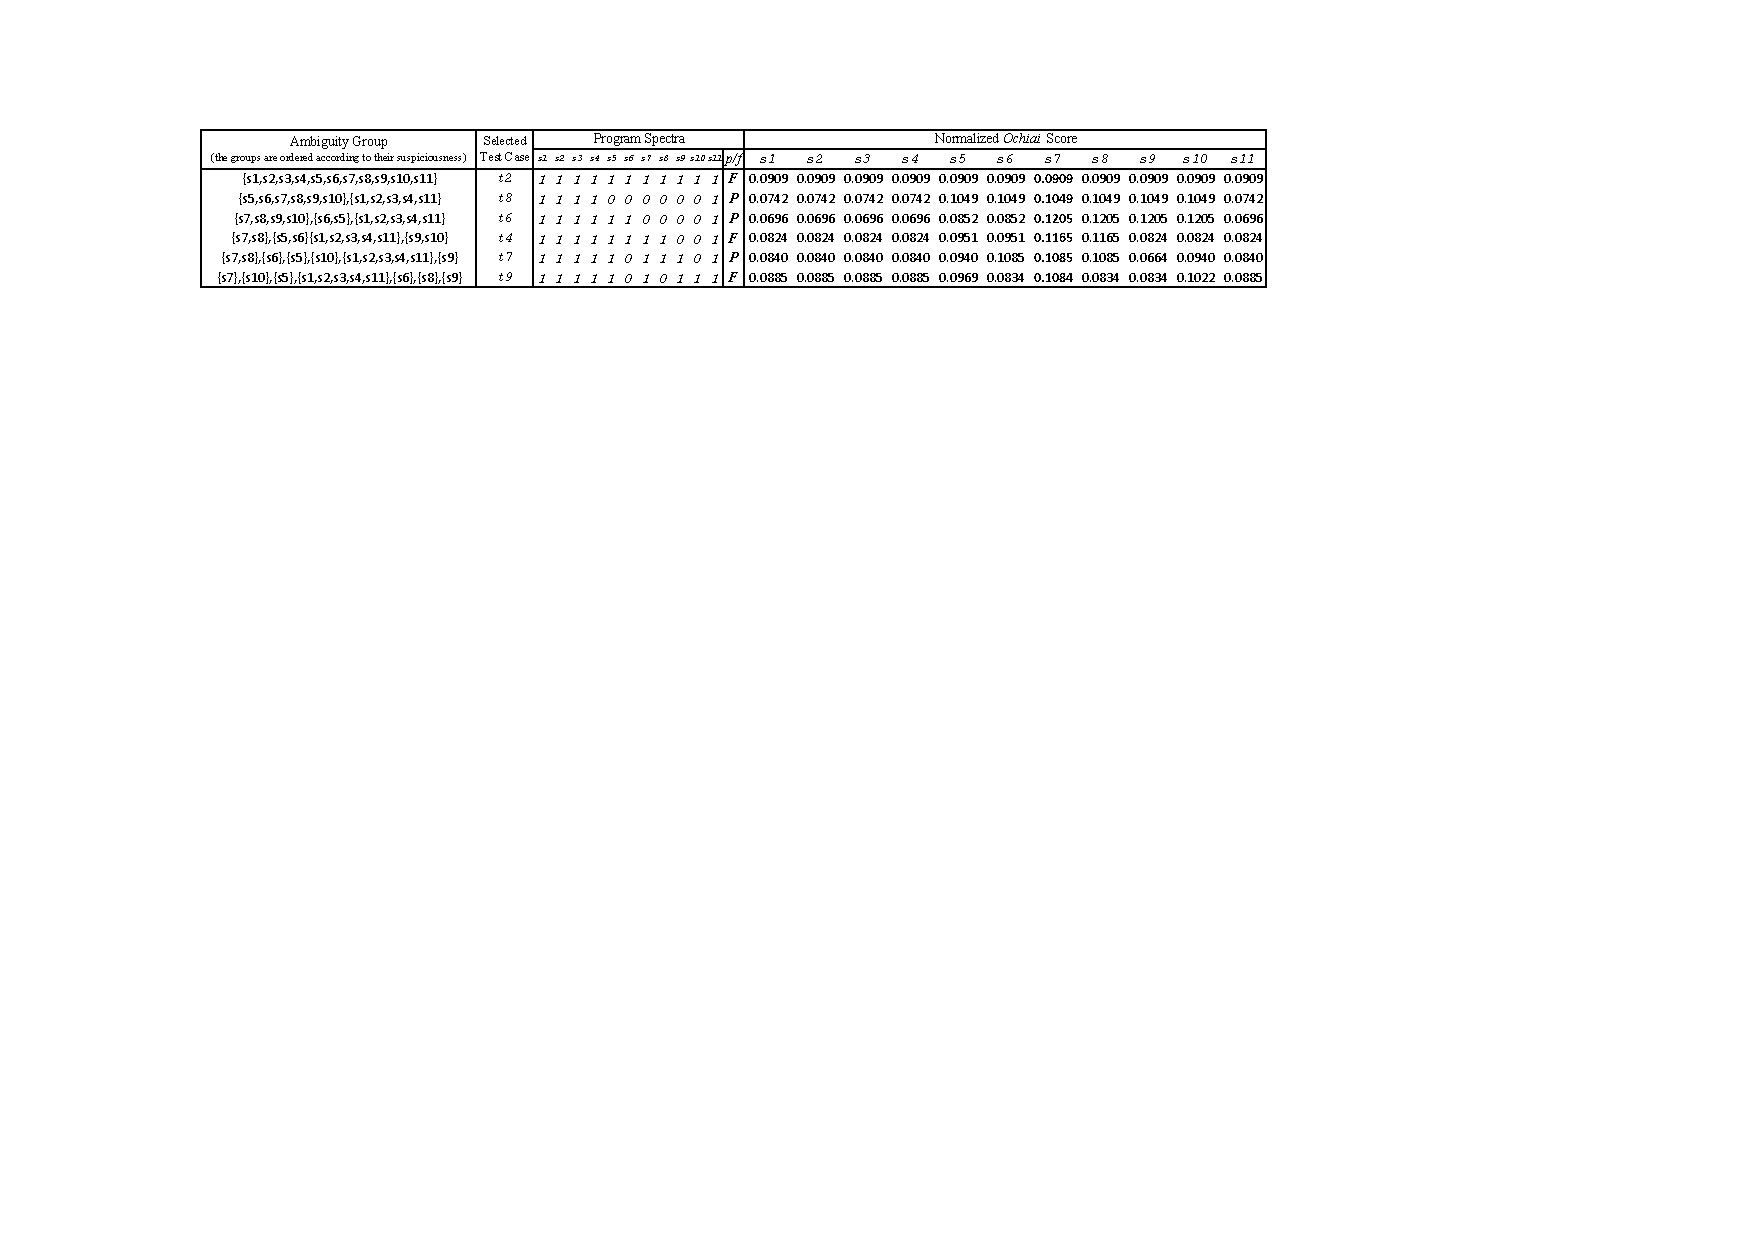
\includegraphics[width=12cm]{ag_table.pdf}
	%\vspace*{-16pt}
    \label{tab:ag_evo}
\end{table}


\begin{algorithm}%[!htb]
{
\centering
%\vspace{0.2cm}
 
\hspace{-0.0cm}\parbox[l]{3.2in} {
{%\small
\begin {tabular}[t]{l}
\textbf{Procedure DiversityMaximizationSpeedup}\\
\textbf{Input:}\\
\quad $k$ - Maximum number of traces to be selected\\
\quad $w$ - Switching threshold\\
\quad $T_\mathcal{U}$ - Unlabeled trace set, where $|T_\mathcal{U}|> k$\\
\quad $t_0$ - Initial failed trace\\
\textbf{Output:}\\
\quad $k$ selected test cases prioritized\\
\textbf{Method:}\\
\end{tabular}
\begin{algorithmic}[1]
	\STATE $T_{tmp} \leftarrow \{<t_0, fail>\}$
	\STATE \textit{\texttt{//Bootstraping with prioritization technique}} $\mathcal{P}$
	\WHILE{$|T_{tmp}|\leq k$ \AND $\left| T_{tmp} \right| \leq w$}
		\STATE Select $t$ by $\mathcal{P}$
		\STATE $c \leftarrow$\texttt{\textbf{manual\_label}}($t$)
		\STATE $T_{tmp} \leftarrow T_{tmp} \cup \left\{\right.<t, c>\left.\right\}$; $T_\mathcal{U}\leftarrow T_\mathcal{U} \setminus \left\{t\right\}$
		\STATE $\forall d \in \mathcal{D}$, calculate suspicious score $f_{T_{tmp}}(d)$
		\STATE $\forall d \in \mathcal{D}$, update trend $\mathcal{T}_{d}$ based on $f_{T_{tmp}}(d)$
	\ENDWHILE
	\STATE $T_\mathcal{S} \leftarrow T_{tmp}$
	\STATE \textit{\texttt{//Speedup}}
	\WHILE{$|T_\mathcal{S}|\leq k$}
		\STATE $\forall d \in \mathcal{D}$, calculate $\mathcal{W}_{\mathcal{T}_{d}}$ by Equation \ref{eq:trend_metric}
		\STATE Select $t$ by Equation \ref{eq:select_metric}
		\STATE $c \leftarrow$\texttt{\textbf{manual\_label}}($t$)
		\STATE $T_{tmp} \leftarrow T_{tmp} \cup \left\{\right.<t, c>\left.\right\}$; $T_\mathcal{U}\leftarrow T_\mathcal{U} \setminus \left\{t\right\}$
		\STATE $\forall d \in \mathcal{D}$, calculate suspicious score $f_{T_{tmp}}(d)$
		\STATE $\forall d \in \mathcal{D}$, update $\mathcal{T}_{d}$ based on $f_{T_{tmp}}(d)$
		\STATE $T_\mathcal{S} \leftarrow T_\mathcal{S} \cup T_{tmp}$
		\IF {\texttt{\textbf{div}}($T_{tmp}$) cease growing}
			\STATE $T_{tmp} \leftarrow \{<t_0, fail>\}$
			\STATE $\forall d \in \mathcal{D}$, clear $\mathcal{T}_{d}$
		\ENDIF
	\ENDWHILE
	\STATE return $T_\mathcal{S}$
\end{algorithmic}
}
}
}
%\vspace{-0.2cm}
\caption{\small{Diversity Maximization Speedup}} \label{algo:DMS}
%\vspace{-0.0cm}
\end{algorithm}











In the pseudocode, \texttt{\textbf{manual\_label}}($t$) asks a user to check
the correctness of the outcome from the test case $t$. Procedure \texttt{\textbf{div}}($T$)
counts the number of unique suspicious scores (diversity) generated by $f_T$, which is defined as follows:
\begin{equation}
	\texttt{\textbf{div}}(T) = \left| \bigcup\limits_{d \in \mathcal{D}} \{f_{T}(d)\} \right|
\end{equation}

The diversity of small programs may reach the maximum after selecting a small number of test cases. To avoid random selection
after that happens, the pseudocode at lines 20-23 resets the set $T_{tmp}$
based on which the suspiciousness scores of all program elements are calculated. With this step, \textsc{Dms} can
continually choose test cases from $T_{\mathcal{U}}$ that maximally diversify suspicious scores calculated based on $T_{tmp}$.
Repeating the diversity selection process also helps to confirm the previously selected test cases and make the final result more robust.

%\lx{merged with the last paragraph in "Example"}
%Table \ref{tab:dms_evo} shows the selected test cases for the motivating example using \textsc{Dms}.  \textsc{Raptor} needs five labeled traces (\texttt{$t_{8}$}$\rightarrow$\texttt{$t_{6}$}$\rightarrow$\texttt{$t_{4}$}$\rightarrow$\texttt{$t_{7}$}$\rightarrow$\texttt{$t_{9}$}) to
%rank the real fault ($s_{7}$) top in the check list (see Table \ref{tab:ag_evo}) based on maximal {\em Ambiguity Group Reduction}(see Section \ref{subsubsec.dp}), \textsc{Dms} only requires user to manually label four traces (\texttt{$t_{8}$}$\rightarrow$\texttt{$t_{6}$}$\rightarrow$\texttt{$t_{4}$}$\rightarrow$\texttt{$t_{9}$}).

%The delay between each round of query is short as the time complexity of computing suspiciousness score for all program elements $\mathcal{D}$ is $O(\left|\mathcal{D}\right|)$ and the time complexity of computing trend score is $O(\left|\mathcal{D}\right| \cdot k)$. Users can choose to stop the process when the cost budget is exhausted (e.g., when the number ($k$) of test cases a user is willing or able to label has been reached).

%Our approach greedily splits suspicious groups based on all previously labeled tests. This may lead to a non-optimal solution as defined by Definition 3.1, but it much simplifies our solution and our empirical study shows it produces promising results to save much human labeling effort, although it may not necessarily save machine time that is required to run all test cases.

%\vspace{0.2cm}
%\noindent{\it Example.}
\subsection{Example}
We describe step by step how \textsc{Dms} minimizes the number of test cases needed by {\em Ochiai} to locate
the fault in the running example in Figure~\ref{motiv_example} and Figure~\ref{tab:dms_evo}.

Since the example code snippet is quite small, there is no need to use a large number of initial test cases to bootstrap our trend analysis. %faulty element $s_{7}$ are ranked $1^{st}$ after selecting only a few traces using \textsc{Raptor}.
We set $w=1$ and only use one test case (in addition to $t_0$) for bootstrapping. In this example and our evaluation in Section~\ref{sec.experiment}, we use \textsc{Raptor}, one of the previously best techniques, in the bootstrapping process for better comparison.

Initially, users execute the program and expose a failure ($t_2$ in this example) in which all statements are covered.
Thus all statements get equal non-zero suspiciousness and constitute a suspicious group $g$. All non-zero suspicious groups compose a group set $G = \{g\}$.
{\sc Raptor} would then choose $t_8$\footnote{$t_8$ has the maximum ambiguity reduction values.} and ask developer to label ({\em pass} or {\em fail}).


After the bootstrapping stage, {\em Ochiai} updates the suspiciousness score for each statement based on the selected traces
and the existing suspicious group set are broken into \{$s_{1}$,$s_{2}$,$s_{3}$,$s_{4}$,$s_{11}$\} and \{$s_{5}$,$s_{6}$,$s_{7}$,$s_{8}$,$s_{9}$,$s_{10}$\}, they are
called $g_{1}$ and $g_{2}$ respectively.
At this time, the trend for the statements in $g_{1}$ is {\bf\texttt{[+]}}, because the ranks of these statements change from 11 to 6, while the trend for the statements in $g_{2}$
is {\bf\texttt{[0]}}, because their ranks are still 11.
The corresponding time series of the statements in $g_{2}$ are:
$y_{0} = 0$ and $ y_{1} = 1$. Applying equation \ref{eq:trend_metric}, we obtain the change-potential of the trend of the program elements in $g_{2}$ as 1.


We now calculate $\mathcal{H}_{G}$ for the current suspicious group set $G=\{g_{1},g_{2}\}$ according to Equation \ref{eq:elem_potential}:

\[\mathcal{H}_{G} = \mathcal{W}_{g_{1}}^{2} + \mathcal{W}_{g_{2}}^{2}  = (\sum_{d \in g_{1}}{0})^{2} + (\sum_{d \in g_{2}}{1})^{2} = 36\].

Now there are 10 candidate traces: $\{t_{i} | 1\leq~i~\leq~12 \wedge i\notin\{2,8\}\}$ to be evaluated. We will use each candidate trace $t_{i}$ to
break ties in $G$ ($G \Leftarrow t_{i}$). Then we calculate the score that evaluates the breaking effect: $\mathcal{H}_{(G \Leftarrow t_{i})}$.

For example, when evaluating $t_6$, $t_{6}$ covers $s_{1}$,$s_{2}$,$s_{3}$,$s_{4}$,$s_{5}$,$s_{6}$ and $s_{11}$, thus breaks suspicious $g_{2}$
into \{$s_{5}$,$s_{6}$\} and \{$s_{7}$,$s_{8}$,$s_{9}$, $s_{10}$\}, let us call them $g_{21}$ and $g_{22}$ respectively.
Now, the score $\mathcal{W}_{g_{21}} = \frac{2}{6} \times \mathcal{W}_{g} = 2$, $\mathcal{W}_{g_{22}} = \frac{4}{6} \times 6 = 4$.
So if choosing $t_{6}$, the score for $G$ is 

\[\mathcal{H}_{(G \Leftarrow t_{6})} = \mathcal{W}_{g_{21}}^{2} + \mathcal{W}_{g_{22}}^{2} = 20\]
And the reduction is 

\[\mathcal{H}_{G} - \mathcal{H}_{(G \Leftarrow t_{6})} = 36 - 20 = 16\].

In the same way, we evaluate all candidate traces and find that the reduction of $t_{6}$ is maximal, so we select $t_{6}$ as the next trace and ask developer to manually label $t_{6}$.
The developer then labels it as {\em ``pass''}.  After adding newly labeled trace $t_{6}$ into the selected trace set $T_{\mathcal{S}}$, we recalculate the suspicious score
of all program elements according to the current selected trace set. After calculation, the normalized suspicious score of the elements in \{$s_{5}$,$s_{6}$\} reduced from 0.1049 to 0.0852 and their ranks remains the same. The suspicious scores of
the elements in \{$s_{7}$,$s_{8}$,$s_{9}$,$s_{10}$\} increase from 0.1049 to 0.1205 and thus their ranks rises from 6 to 4. After that, the trends of program elements are updated. For example, the trend of elements in \{$s_{1}$,$s_{2}$,$s_{3}$,$s_{4}$,$s_{13}$\} becomes ({\bf\texttt{[0]}}{\bf\texttt{[0]}}), the trend
of the statements in \{$s_{5}$,$s_{6}$\} becomes ({\bf\texttt{[+]}}{\bf\texttt{[0]}}) and those in \{$s_{7}$,$s_{8}$,$s_{9}$,$s_{10}$\} corresponds to ({\bf\texttt{[+]}}{\bf\texttt{[+]}}).


Note that right now \{$s_{7}$,$s_{8}$,$s_{9}$,$s_{10}$\} gets the highest change-potential score and thus can get more chances to be broken up.
As shown in Table \ref{tab:dms_evo},
after three iterations,
\textsc{Dms} selects (\texttt{$t_{8}$}$\rightarrow$\texttt{$t_{6}$}$\rightarrow$\texttt{$t_{4}$}). In the next iteration, \textsc{Dms} chooses $t_{9}$ and breaks \{$s_{7}$,$s_{8}$\} and \{$s_{5}$,$s_{6}$\} which have greater change-potentials and consequently ranks $s_7$ the highest. Overall, {\sc Dms} only requires user to manually label four additional traces (\texttt{$t_{8}$}$\rightarrow$\texttt{$t_{6}$}$\rightarrow$\texttt{$t_{4}$}$\rightarrow$\texttt{$t_{9}$}).

As a comparison, \textsc{Raptor} always chooses the test case that maximally reduces the overall sizes of groups of statements that have the spectrum records (i.e., Ambiguity Group Reduction, c.f.\ Section~\ref{subsubsec.dp}). As shown in Table~\ref{tab:ag_evo}, \textsc{Raptor} effectively selects the same test cases as {\sc Dms} in the first four iterations; however, it chooses $t_{7}$ in the next iteration to break \{$s_{1}$,$s_{2}$,$s_{3}$,$s_{4}$,$s_{9}$,$s_{10}$,$s_{11}$\} and \{$s_{5}$,$s_{6}$\}, and it takes one more iteration to rank $s_7$ the highest.
%Because breaking these groups can get maximal overall group size reduction.
It thus requires users to label five additional test cases besides $t_2$ (\texttt{$t_{8}$}$\rightarrow$\texttt{$t_{6}$}$\rightarrow$\texttt{$t_{4}$}$\rightarrow$\texttt{$t_{7}$}$\rightarrow$\texttt{$t_{9}$}).

